\chapter{L16 -- Osservabilità, forma standard di osservabilità e decomposizione di Kalman}
\label{chap:L16}

\section{Idea generale della lezione}

In questa lezione completiamo il quadro iniziato nelle lezioni precedenti su:
\begin{itemize}
    \item sottospazio di inosservabilità;
    \item forma standard di osservabilità;
    \item criterio PBH per l'osservabilità;
    \item relazione tra autovalori, osservabilità e poli della funzione di trasferimento;
    \item decomposizione canonica di Kalman;
    \item interpretazione dei modi del sistema in termini di raggiungibilità e osservabilità.
\end{itemize}

L'idea di fondo è la seguente:

\begin{quote}
\emph{non tutti gli autovalori della matrice di stato \(A\) compaiono necessariamente nella funzione di trasferimento \(G(s)\): compaiono solo i modi che sono sia raggiungibili sia osservabili.}
\end{quote}

Questo è il cuore della lezione.

\bigskip

\section{Parte osservabile e parte inosservabile}

Ricordiamo che, per un sistema lineare stazionario

\[
\Sigma:
\begin{cases}
\dot x = Ax + Bu \\
y = Cx + Du
\end{cases}
\qquad\text{(tempo continuo)}
\]

oppure

\[
\Sigma:
\begin{cases}
x(k+1) = Ax(k) + Bu(k) \\
y(k) = Cx(k) + Du(k)
\end{cases}
\qquad\text{(tempo discreto)},
\]

il \emph{sottospazio di inosservabilità} è

\[
\bar{\mathcal O}
=
\ker(\mathcal O)
=
\bigcap_{i=0}^{n-1}\ker(CA^i),
\]

dove

\[
\mathcal O=
\begin{bmatrix}
C \\ CA \\ CA^2 \\ \vdots \\ CA^{n-1}
\end{bmatrix}
\]

è la matrice di osservabilità.

\medskip

Il significato geometrico è il seguente:

\begin{itemize}
    \item se \(x_0\in\bar{\mathcal O}\), allora l'evoluzione libera a partire da \(x_0\) non produce alcun effetto misurabile in uscita;
    \item quindi \(\bar{\mathcal O}\) raccoglie tutti gli stati che il sensore non riesce a distinguere dall'origine;
    \item inoltre \(\bar{\mathcal O}\) è il più grande sottospazio \(A\)-invariante contenuto in \(\ker(C)\).
\end{itemize}

\medskip

Scegliendo una base adattata a \(\bar{\mathcal O}\), il sistema può essere scritto in \emph{forma standard di osservabilità}:

\[
T^{-1}AT=
\begin{bmatrix}
A_o & 0 \\
A_{\bar o,o} & A_{\bar o}
\end{bmatrix},
\qquad
T^{-1}B=
\begin{bmatrix}
B_o \\ B_{\bar o}
\end{bmatrix},
\qquad
CT=
\begin{bmatrix}
C_o & 0
\end{bmatrix},
\qquad
D=\tilde D.
\]

Qui:
\begin{itemize}
    \item \(A_o\) descrive la \emph{parte osservabile};
    \item \(A_{\bar o}\) descrive la \emph{parte inosservabile};
    \item l'uscita dipende solo dalle coordinate associate alla parte osservabile.
\end{itemize}

\section{Autovalori osservabili e funzione di trasferimento}

Nella forma standard di osservabilità si ha

\[
G(s)=C(sI-A)^{-1}B + D.
\]

Sostituendo la struttura a blocchi precedente:

\[
sI-\tilde A=
\begin{bmatrix}
sI-A_o & 0 \\
-A_{\bar o,o} & sI-A_{\bar o}
\end{bmatrix}.
\]

Essendo questa matrice triangolare a blocchi inferiori, la sua inversa ha la forma

\[
(sI-\tilde A)^{-1}
=
\begin{bmatrix}
(sI-A_o)^{-1} & 0 \\
\ast & (sI-A_{\bar o})^{-1}
\end{bmatrix}.
\]

Di conseguenza

\[
G(s)
=
\begin{bmatrix}
C_o & 0
\end{bmatrix}
\begin{bmatrix}
(sI-A_o)^{-1} & 0 \\
\ast & (sI-A_{\bar o})^{-1}
\end{bmatrix}
\begin{bmatrix}
B_o \\ B_{\bar o}
\end{bmatrix}
+ D
=
C_o(sI-A_o)^{-1}B_o + D.
\]

Questa formula è fondamentale: la funzione di trasferimento \emph{non dipende} dal blocco \(A_{\bar o}\).

\medskip

Quindi:

\begin{quote}
\emph{Gli autovalori del blocco inosservabile \(A_{\bar o}\) non compaiono nella funzione di trasferimento.}
\end{quote}

Equivalentemente, i poli della funzione di trasferimento sono legati solo agli autovalori osservabili.

\medskip

Se il sistema originario ha ordine \(n\), ma la parte osservabile ha dimensione \(n-\bar o\), allora nella funzione di trasferimento il denominatore effettivo ha grado \(n-\bar o\): ciò significa che sono avvenute cancellazioni polo-zero.

\bigskip

\section{Interpretazione: perché compaiono cancellazioni?}

Supponiamo che il sistema completo abbia polinomio caratteristico

\[
\chi_A(s)=\det(sI-A)
\]

di grado \(n\). Se una parte degli autovalori è inosservabile, allora nella funzione di trasferimento non compaiono tutti i modi del sistema, ma solo quelli effettivamente ``visibili'' dall'uscita.

Perciò si può avere

\[
G(s)=\frac{m(s)}{d(s)}, \qquad \deg d(s)=n-\bar o<n.
\]

In altre parole:
\begin{itemize}
    \item il modello di stato ha un certo ordine;
    \item la funzione di trasferimento può avere ordine minore;
    \item la differenza è dovuta a modi interni nascosti, cioè non osservabili.
\end{itemize}

\bigskip

\section{Lemma PBH per l'osservabilità}

Esiste un criterio molto comodo, duale di quello di raggiungibilità.

\medskip

\noindent\textbf{Lemma di Popov-Belevitch-Hautus (PBH) per l'osservabilità.}

La coppia \((A,C)\) è osservabile se e solo se

\[
\operatorname{rank}
\begin{bmatrix}
\lambda I-A\\
C
\end{bmatrix}
= n
\qquad \forall \lambda\in\mathbb C.
\]

In forma equivalente, trasponendo,

\[
\operatorname{rank}
\begin{bmatrix}
\lambda I-A^T & C^T
\end{bmatrix}
= n
\qquad \forall \lambda\in\mathbb C.
\]

\medskip

\noindent\textbf{Interpretazione.}
Se per un certo autovalore \(\lambda\) il rango scende, allora esiste un vettore non nullo \(v\neq 0\) tale che

\[
(\lambda I-A)v=0,
\qquad
Cv=0.
\]

La prima relazione dice che \(v\) è un autovettore associato a \(\lambda\), mentre la seconda dice che quell'autodirezione è invisibile in uscita.  
Quindi il modo \(\lambda\) non è osservabile.

\medskip

\noindent\textbf{Lettura concettuale del lemma.}
\begin{quote}
\emph{Un sistema è osservabile se nessun autovettore di \(A\) è annullato da \(C\).}
\end{quote}

Quando ci sono autovalori multipli o blocchi di Jordan non banali, il criterio PBH è ancora più utile della sola matrice di osservabilità, perché consente di capire subito quali modi sono nascosti.

\section{Un primo esempio: osservabilità con più o meno sensori}

Consideriamo

\[
A=
\begin{bmatrix}
2 & 1 & 0\\
-1 & 0 & 1\\
0 & 2 & 1
\end{bmatrix},
\qquad
C=
\begin{bmatrix}
1 & 0 & 0\\
0 & 1 & 0
\end{bmatrix}.
\]

La matrice di osservabilità è

\[
\mathcal O=
\begin{bmatrix}
C\\
CA\\
CA^2
\end{bmatrix}.
\]

Poiché

\[
CA=
\begin{bmatrix}
2 & 1 & 0\\
-1 & 0 & 1
\end{bmatrix},
\]

già le righe di \(C\) e la seconda riga di \(CA\) sono linearmente indipendenti; quindi si ottiene rango \(3\), e il sistema è completamente osservabile.

\medskip

Ora supponiamo invece di usare un solo sensore:

\[
C_1=
\begin{bmatrix}
1 & 0 & 0
\end{bmatrix}.
\]

Allora

\[
\mathcal O_1=
\begin{bmatrix}
C_1\\
C_1A\\
C_1A^2
\end{bmatrix}
=
\begin{bmatrix}
1 & 0 & 0\\
2 & 1 & 0\\
3 & 2 & 1
\end{bmatrix}.
\]

Si vede immediatamente che \(\mathcal O_1\) è triangolare inferiore con diagonale non nulla, dunque

\[
\det(\mathcal O_1)=1\neq 0,
\]

e quindi anche con un solo sensore il sistema resta completamente osservabile.

\medskip

Questo esempio mostra una cosa importante:

\begin{quote}
\emph{non è vero che serva necessariamente misurare tutte le componenti di stato; basta che le uscite contengano informazione sufficiente a ricostruire lo stato.}
\end{quote}

\bigskip

\section{Esempio fondamentale: sistema raggiungibile ma non osservabile}

Consideriamo ora

\[
A=
\begin{bmatrix}
2 & 1 & 0\\
1 & 0 & 0\\
0 & 2 & 1
\end{bmatrix},
\qquad
B=
\begin{bmatrix}
0\\
1\\
0
\end{bmatrix},
\qquad
C=
\begin{bmatrix}
1 & 1 & 0
\end{bmatrix}.
\]

\subsection{Studio dell'osservabilità}

La matrice di osservabilità è

\[
\mathcal O=
\begin{bmatrix}
C\\
CA\\
CA^2
\end{bmatrix}.
\]

Calcoliamo:

\[
CA=
\begin{bmatrix}
3 & 1 & 0
\end{bmatrix},
\qquad
CA^2=
\begin{bmatrix}
7 & 3 & 0
\end{bmatrix}.
\]

Dunque

\[
\mathcal O=
\begin{bmatrix}
1 & 1 & 0\\
3 & 1 & 0\\
7 & 3 & 0
\end{bmatrix}.
\]

La terza colonna è nulla, quindi

\[
\operatorname{rank}(\mathcal O)=2.
\]

Il sistema non è completamente osservabile.  
Inoltre

\[
\bar{\mathcal O}
=
\ker(\mathcal O)
=
\operatorname{span}\left\{
\begin{bmatrix}
0\\0\\1
\end{bmatrix}
\right\}.
\]

Quindi la direzione \(e_3\) è inosservabile.

\subsection{Studio della raggiungibilità}

La matrice di raggiungibilità è

\[
\mathcal R=
\begin{bmatrix}
B & AB & A^2B
\end{bmatrix}.
\]

Si calcola:

\[
AB=
\begin{bmatrix}
1\\0\\2
\end{bmatrix},
\qquad
A^2B=
\begin{bmatrix}
2\\1\\2
\end{bmatrix},
\]

per cui

\[
\mathcal R=
\begin{bmatrix}
0 & 1 & 2\\
1 & 0 & 1\\
0 & 2 & 2
\end{bmatrix}.
\]

Si verifica che

\[
\operatorname{rank}(\mathcal R)=3,
\]

quindi il sistema è completamente raggiungibile.

\subsection{Conclusione}

Abbiamo dunque una situazione molto istruttiva:

\[
\text{sistema completamente raggiungibile, ma non completamente osservabile.}
\]

Questo significa che:
\begin{itemize}
    \item con l'ingresso posso eccitare tutti i modi;
    \item ma uno di questi modi non viene visto in uscita.
\end{itemize}

\subsection{Verifica immediata con PBH}

L'autovalore \(\lambda=1\) è chiaramente un autovalore di \(A\), perché

\[
Ae_3=e_3,
\qquad
Ce_3=0.
\]

Quindi il modo \(\lambda=1\) è inosservabile.  
Infatti

\[
\operatorname{rank}
\begin{bmatrix}
I-A\\
C
\end{bmatrix}
<3.
\]

\subsection{Il sistema è già in forma standard di osservabilità}

Osserviamo che \(e_3\) è proprio l'ultima coordinata, e la matrice \(A\) ha la forma

\[
A=
\begin{bmatrix}
2 & 1 & 0\\
1 & 0 & 0\\
0 & 2 & 1
\end{bmatrix}
=
\left[
\begin{array}{c|c}
A_o & 0\\
\hline
A_{\bar o,o} & A_{\bar o}
\end{array}
\right]
\]

con

\[
A_o=
\begin{bmatrix}
2 & 1\\
1 & 0
\end{bmatrix},
\qquad
A_{\bar o,o}=
\begin{bmatrix}
0 & 2
\end{bmatrix},
\qquad
A_{\bar o}=
\begin{bmatrix}
1
\end{bmatrix}.
\]

Inoltre

\[
B=
\begin{bmatrix}
0\\1\\0
\end{bmatrix}
=
\begin{bmatrix}
B_o\\
B_{\bar o}
\end{bmatrix},
\qquad
B_o=
\begin{bmatrix}
0\\1
\end{bmatrix},
\quad
B_{\bar o}=0,
\]

e

\[
C=
\begin{bmatrix}
1 & 1 & 0
\end{bmatrix}
=
\begin{bmatrix}
C_o & 0
\end{bmatrix},
\qquad
C_o=
\begin{bmatrix}
1 & 1
\end{bmatrix}.
\]

Perciò la funzione di trasferimento dipende solo dal blocco osservabile \(A_o\):

\[
G(s)=C_o(sI-A_o)^{-1}B_o.
\]

Calcolando si ottiene

\[
G(s)=\frac{s-1}{s^2-2s-1}.
\]

D'altra parte il polinomio caratteristico della matrice completa \(A\) è

\[
\chi_A(s)=\det(sI-A)=(s-1)(s^2-2s-1).
\]

Quindi il polo \(s=1\), associato al modo inosservabile, si cancella.

\medskip

Questo esempio riassume perfettamente il significato della lezione:

\begin{quote}
\emph{un autovalore può essere presente nello stato ma assente nella funzione di trasferimento, se è inosservabile.}
\end{quote}

\bigskip

\section{Forma canonica di osservabilità}

Per sistemi SISO strettamente propri, la forma canonica di osservabilità è la trasposta della forma canonica di controllo.

Supponiamo di avere una funzione di trasferimento

\[
G(s)=
\frac{b_0+b_1s+\cdots+b_ps^p}
{s^n+a_{n-1}s^{n-1}+\cdots+a_1s+a_0},
\qquad p<n.
\]

Una realizzazione canonica osservabile è

\[
A_o=
\begin{bmatrix}
0 & 0 & \cdots & 0 & -a_0\\
1 & 0 & \cdots & 0 & -a_1\\
0 & 1 & \cdots & 0 & -a_2\\
\vdots & \vdots & \ddots & \vdots & \vdots\\
0 & 0 & \cdots & 1 & -a_{n-1}
\end{bmatrix},
\]

\[
B_o=
\begin{bmatrix}
b_0\\
b_1\\
\vdots\\
b_p\\
0\\
\vdots\\
0
\end{bmatrix},
\qquad
C_o=
\begin{bmatrix}
0 & 0 & \cdots & 0 & 1
\end{bmatrix},
\qquad
D=0.
\]

\medskip

Questa forma è utile perché:
\begin{itemize}
    \item è \emph{sempre completamente osservabile};
    \item rappresenta direttamente la funzione di trasferimento;
    \item è duale della forma canonica di controllo.
\end{itemize}

\section{Dualità tra raggiungibilità e osservabilità}

La dualità è un principio chiave.

Consideriamo il sistema originario

\[
\Sigma:
\begin{cases}
x^+ = Ax + Bu \\
y = Cx + Du
\end{cases}
\]

e il sistema duale

\[
\Sigma^d:
\begin{cases}
z^+ = A^Tz + C^Tv \\
w = B^Tz + D^Tv.
\end{cases}
\]

Allora:
\begin{itemize}
    \item la raggiungibilità del sistema duale corrisponde all'osservabilità del sistema originario;
    \item la matrice di raggiungibilità del duale è la trasposta della matrice di osservabilità dell'originale.
\end{itemize}

Infatti

\[
\mathcal R_d=
\begin{bmatrix}
C^T & A^TC^T & (A^T)^2C^T & \cdots & (A^T)^{n-1}C^T
\end{bmatrix}
=
\mathcal O^T.
\]

Quindi

\[
(A,C)\ \text{osservabile}
\iff
(A^T,C^T)\ \text{raggiungibile}.
\]

Questa osservazione spiega perché:
\begin{itemize}
    \item la forma standard di osservabilità è la versione duale della forma standard di raggiungibilità;
    \item il lemma PBH per l'osservabilità si ottiene trasponendo quello per la raggiungibilità;
    \item la forma canonica di osservabilità è la trasposta della forma canonica di controllo.
\end{itemize}

\bigskip

\section{Decomposizione canonica di Kalman}

La forma standard di raggiungibilità separa:
\[
\mathcal R \quad\text{e}\quad \bar{\mathcal R},
\]
mentre la forma standard di osservabilità separa:
\[
\mathcal O \quad\text{e}\quad \bar{\mathcal O}.
\]

Se vogliamo tenere conto \emph{simultaneamente} di entrambe le proprietà, dobbiamo combinare le due decomposizioni.

\medskip

L'idea è considerare i quattro tipi di modi:
\begin{enumerate}
    \item raggiungibili e osservabili;
    \item raggiungibili ma non osservabili;
    \item non raggiungibili ma osservabili;
    \item non raggiungibili e non osservabili.
\end{enumerate}

\subsection{Schema geometrico}

\begin{center}
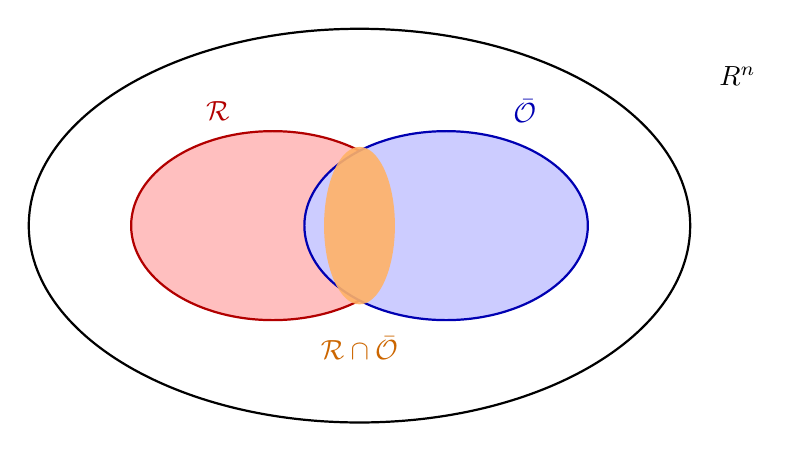
\begin{tikzpicture}[scale=1.0]
    \draw[thick] (0,0) ellipse (4.2 and 2.5);
    \node at (4.8,1.9) {$\mathbb R^n$};

    \fill[red!25] (-1.1,0) ellipse (1.8 and 1.2);
    \draw[thick,red!70!black] (-1.1,0) ellipse (1.8 and 1.2);
    \node[red!70!black] at (-1.8,1.45) {$\mathcal R$};

    \fill[blue!20] (1.1,0) ellipse (1.8 and 1.2);
    \draw[thick,blue!70!black] (1.1,0) ellipse (1.8 and 1.2);
    \node[blue!70!black] at (2.1,1.45) {$\bar{\mathcal O}$};

    \fill[orange!60,opacity=0.9] (0,0) ellipse (0.45 and 1.0);
    \node[orange!80!black] at (0,-1.55) {$\mathcal R\cap\bar{\mathcal O}$};
\end{tikzpicture}
\end{center}

\medskip

Il primo passo pratico è costruire una base di \(\mathcal R\cap\bar{\mathcal O}\).  
Poi si completa:
\begin{itemize}
    \item dentro \(\mathcal R\);
    \item dentro \(\bar{\mathcal O}\);
    \item infine in tutto lo spazio di stato.
\end{itemize}

\subsection{Forma strutturale}

Esiste allora un cambio di coordinate \(x=Tz\) tale che il sistema assuma una forma a quattro blocchi.  
A seconda dell'ordine scelto nella base, la disposizione dei blocchi può cambiare; una forma tipica è

\[
\tilde A=
\begin{bmatrix}
A_{RO} & * & * & *\\
0 & A_{R\bar O} & * & *\\
0 & 0 & A_{\bar R O} & *\\
0 & 0 & 0 & A_{\bar R\bar O}
\end{bmatrix},
\qquad
\tilde B=
\begin{bmatrix}
B_{RO}\\
B_{R\bar O}\\
0\\
0
\end{bmatrix},
\qquad
\tilde C=
\begin{bmatrix}
C_{RO} & 0 & C_{\bar R O} & 0
\end{bmatrix}.
\]

La lettura è immediata:
\begin{itemize}
    \item l'ingresso agisce solo sui blocchi raggiungibili;
    \item l'uscita vede solo i blocchi osservabili;
    \item il blocco veramente rilevante per la dinamica ingresso--uscita è quello \emph{raggiungibile e osservabile}, cioè \(A_{RO}\).
\end{itemize}

\subsection{Riduzione della funzione di trasferimento}

La conseguenza più importante è:

\[
G(s)=C_{RO}(sI-A_{RO})^{-1}B_{RO}+D.
\]

Quindi i poli di \(G(s)\) sono esattamente gli autovalori del blocco \(A_{RO}\), cioè:

\begin{quote}
\emph{i modi che sono contemporaneamente raggiungibili e osservabili.}
\end{quote}

\section{Riassunto dei modi che compaiono}

Per fissare bene le idee, è utile distinguere quattro livelli.

\begin{center}
\renewcommand{\arraystretch}{1.4}
\begin{tabular}{|c|c|c|}
\hline
\textbf{Oggetto studiato} & \textbf{Modi che compaiono} & \textbf{Commento} \\
\hline
Stato libero \(x(t)\) & autovalori di \(A\) & tutti i modi interni \\
\hline
Stato forzato & autovalori raggiungibili di \(A\) & solo quelli eccitabili dall'ingresso \\
\hline
Uscita libera \(y(t)\) & autovalori osservabili di \(A\) & solo quelli visibili dal sensore \\
\hline
Funzione di trasferimento \(G(s)\) & autovalori sia raggiungibili sia osservabili & modi ingresso--uscita \\
\hline
\end{tabular}
\end{center}

\medskip

Questo schema è una delle sintesi più importanti di tutto il corso.

\bigskip

\section{Esempio finale: raggiungibile e non osservabile}

Riprendiamo l'esempio

\[
A=
\begin{bmatrix}
2 & 1 & 0\\
1 & 0 & 0\\
0 & 2 & 1
\end{bmatrix},
\qquad
B=
\begin{bmatrix}
0\\1\\0
\end{bmatrix},
\qquad
C=
\begin{bmatrix}
1 & 1 & 0
\end{bmatrix}.
\]

Abbiamo trovato:

\[
\mathcal R=\mathbb R^3,
\qquad
\bar{\mathcal O}
=
\operatorname{span}\left\{
\begin{bmatrix}
0\\0\\1
\end{bmatrix}
\right\}.
\]

Poiché \(\mathcal R=\mathbb R^3\), si ha

\[
\mathcal R\cap\bar{\mathcal O}
=
\bar{\mathcal O}
=
\operatorname{span}\left\{
\begin{bmatrix}
0\\0\\1
\end{bmatrix}
\right\}.
\]

Quindi:
\begin{itemize}
    \item esiste una parte raggiungibile ma non osservabile;
    \item non esiste una parte non raggiungibile;
    \item la decomposizione di Kalman qui si riduce di fatto alla forma standard di osservabilità.
\end{itemize}

In particolare il sistema è già scritto come

\[
A=
\left[
\begin{array}{c|c}
A_o & 0\\
\hline
A_{\bar o,o} & A_{\bar o}
\end{array}
\right],
\qquad
C=
\begin{bmatrix}
C_o & 0
\end{bmatrix},
\]

con

\[
A_o=
\begin{bmatrix}
2 & 1\\
1 & 0
\end{bmatrix},
\qquad
A_{\bar o}=
\begin{bmatrix}
1
\end{bmatrix}.
\]

Perciò il modo \(1\) rimane nello stato ma scompare dalla funzione di trasferimento.

\bigskip

\section{Osservazione finale}

Le due forme standard che abbiamo costruito nel corso hanno significati complementari:

\begin{itemize}
    \item \textbf{Forma standard di raggiungibilità (FSR):} separa ciò che l'ingresso può muovere da ciò che non può muovere.
    \item \textbf{Forma standard di osservabilità (FSO):} separa ciò che l'uscita riesce a vedere da ciò che non riesce a vedere.
\end{itemize}

La \textbf{decomposizione di Kalman} sovrappone queste due informazioni e separa completamente:
\begin{itemize}
    \item parte raggiungibile e osservabile;
    \item parte raggiungibile e non osservabile;
    \item parte non raggiungibile e osservabile;
    \item parte non raggiungibile e non osservabile.
\end{itemize}

La morale è:

\begin{quote}
\emph{dal punto di vista ingresso--uscita conta solo la parte minima del sistema, cioè quella contemporaneamente raggiungibile e osservabile.}
\end{quote}

Tutto il resto è dinamica interna nascosta: può esistere nello stato, ma non compare nella funzione di trasferimento.

\bigskip

\section*{Promemoria operativo per gli esercizi}

Quando in un compito devi studiare osservabilità e poli della funzione di trasferimento, conviene seguire questa scaletta:

\begin{enumerate}
    \item calcolare \(\mathcal O\) e il suo rango;
    \item ricavare \(\bar{\mathcal O}=\ker(\mathcal O)\);
    \item se utile, verificare i modi inosservabili con PBH;
    \item cercare una base adattata a \(\bar{\mathcal O}\) per scrivere la FSO;
    \item leggere il blocco osservabile \(A_o\);
    \item concludere che i poli della FDT sono gli autovalori del blocco osservabile;
    \item se serve combinare tutto con la raggiungibilità, passare alla decomposizione di Kalman.
\end{enumerate}